\documentclass[14pt]{chalkfjord}

\includeonlyframes{distributive-law}

\usepackage{ulem}
\usetikzlibrary{matrix,arrows}
\usetikzlibrary{calc}
\usetikzlibrary{intersections}
\usetikzlibrary{through,positioning}
\usetikzlibrary{decorations.markings}

\usetikzlibrary{calc,fadings,decorations.pathreplacing}
%% helper macros

\newcommand\pgfmathsinandcos[3]{%
  \pgfmathsetmacro#1{sin(#3)}%
  \pgfmathsetmacro#2{cos(#3)}%
}
\newcommand\LongitudePlane[3][current plane]{%
  \pgfmathsinandcos\sinEl\cosEl{#2} % elevation
  \pgfmathsinandcos\sint\cost{#3} % azimuth
  \tikzset{#1/.estyle={cm={\cost,\sint*\sinEl,0,\cosEl,(0,0)}}}
}
\newcommand\LatitudePlane[3][current plane]{%
  \pgfmathsinandcos\sinEl\cosEl{#2} % elevation
  \pgfmathsinandcos\sint\cost{#3} % latitude
  \pgfmathsetmacro\yshift{\cosEl*\sint}
  \tikzset{#1/.estyle={cm={\cost,0,0,\cost*\sinEl,(0,\yshift)}}} %
}
\newcommand\DrawLongitudeCircle[2][1]{
  \LongitudePlane{\angEl}{#2}
  \tikzset{current plane/.prefix style={scale=#1}}
   % angle of "visibility"
  \pgfmathsetmacro\angVis{atan(sin(#2)*cos(\angEl)/sin(\angEl))} %
  \draw[current plane] (\angVis:1) arc (\angVis:\angVis+180:1);
  \draw[current plane,dashed] (\angVis-180:1) arc (\angVis-180:\angVis:1);
}
\newcommand\DrawLatitudeCircle[2][1]{
  \LatitudePlane{\angEl}{#2}
  \tikzset{current plane/.prefix style={scale=#1}}
  \pgfmathsetmacro\sinVis{sin(#2)/cos(#2)*sin(\angEl)/cos(\angEl)}
  % angle of "visibility"
  \pgfmathsetmacro\angVis{asin(min(1,max(\sinVis,-1)))}
  \draw[current plane] (\angVis:1) arc (\angVis:-\angVis-180:1);
  \draw[current plane,dashed] (180-\angVis:1) arc (180-\angVis:\angVis:1);
}

\usepackage{calc}
\pgfdeclarefading{shinyfade} {\tikz \shade[top color=pgftransparent!40, bottom color=pgftransparent!0] (0,0) rectangle (2,2);}

\newlength{\reflectedtextheight}
\newcommand{\reflectedtext}[1]{%
\settototalheight{\reflectedtextheight}{#1}
\begin{pgfpicture}{0in}{0in}{\textwidth}{1.35\reflectedtextheight}
\pgfsetxvec{\pgfpoint{\textwidth}{0cm}}
\pgfsetyvec{\pgfpoint{0cm}{1.35\reflectedtextheight}}

\pgftransformshift{\pgfxy(0.5,0.35)}
\pgfnode{rectangle}{south}{#1}{}{\pgfusepath{}}

\pgftransformyscale{-0.35}
\pgfnode{rectangle}{south}{#1}{}{}

\pgfsetfadingforcurrentpath{shinyfade}{}
\color{white}
\pgffill

\end{pgfpicture}
}

\newcommand{\setbackgroundpicture}[1]{%
\usebackgroundtemplate{
\begin{pgfpicture}{0in}{0in}{\paperwidth}{\paperheight}
\pgfputat{\pgfxy(0,0)}{\includegraphics[keepaspectratio=false,width=\paperwidth,height=\paperheight]{#1}}
\color{white}
%\pgfsetfillopacity{0.8}
%\pgfrect[fill]{\pgfxy(0,0)}{\pgfpoint{\paperwidth}{\paperheight}}
\end{pgfpicture}
}
}
\newcommand{\setlightbackgroundpicture}[1]{%
\usebackgroundtemplate{
\begin{pgfpicture}{0in}{0in}{\paperwidth}{\paperheight}
\pgfputat{\pgfxy(0,0)}{\includegraphics[keepaspectratio=false,width=\paperwidth,height=\paperheight]{#1}}
\color{white}
\pgfsetfillopacity{0.7}
\pgfrect[fill]{\pgfxy(0,0)}{\pgfpoint{\paperwidth}{\paperheight}}
\end{pgfpicture}
}
}

\newcommand{\setbackgroundblack}{%
\usebackgroundtemplate{
\begin{pgfpicture}{0in}{0in}{\paperwidth}{\paperheight}
\color{black}
\pgfrect[fill]{\pgfxy(0,0)}{\pgfpoint{\paperwidth}{\paperheight}}
\end{pgfpicture}
}
}

\newcommand{\clearbackgroundpicture}{\usebackgroundtemplate{}}

\makeatletter
\define@key{beamerframe}{nofills}[true]{% top
  \beamer@frametopskip=0pt\relax%
  \beamer@framebottomskip=0pt\relax%
  \beamer@frametopskipautobreak=\beamer@frametopskip\relax%
  \beamer@framebottomskipautobreak=\beamer@framebottomskip\relax%
  \def\beamer@initfirstlineunskip{%
    \def\beamer@firstlineitemizeunskip{%
      \vskip-\partopsep\vskip-\topsep\vskip-\parskip%
      \global\let\beamer@firstlineitemizeunskip=\relax}%
    \everypar{\global\let\beamer@firstlineitemizeunskip=\relax}}
}
\makeatother

\newcommand{\Z}{\mathbb{Z}}
\newcommand{\Q}{\mathbb{Q}}
\newcommand{\R}{\mathbb{R}}
\newcommand{\C}{\mathbb{C}}

\author{Jim Fowler}
%\date{April 20, 2011}
\date{October 5, 2013}
\title{Projective Planes}

\newcommand{\quat}[1]{\mathbf{#1}}

%%%%%%%%%%%%%%%%%%%%%%%%%%%%%%%%%%%%%%%%%%%%%%%%%%%%%%%%%%%%%%%%
\begin{document}

%%%%%%%%%%%%%%%%%%%%%%%%%%%%%%%%%%%%%%%%%%%%%%%%%%%%%%%%%%%%%%%%
% nice looking title
\begin{frame}[nofills,label=title]
  \vfill

  \noindent {\Huge\scalebox{1.8}{\textbf{Projective}}} \vspace{-2.2ex}\\
  \noindent\null\hspace{2in}{\Huge\scalebox{1.8}{\textbf{Planes}}}

  \vfill
  \large
  \noindent \textsf{\textbf{Jim Fowler}}\hfill\textsf{The Ohio State University}

  \vfill
  \footnotesize

  \noindent Undergraduate Mathematics Symposium \hfill 5 October 2013 \\
  \noindent at the University of Illinois at Chicago

\end{frame}

\clearbackgroundpicture

%%%%%%%%%%%%%%%%%%%%%%%%%%%%%%%%%%%%%%%%%%%%%%%%%%%%%%%%%%%%%%%%
% geometry versus algebra
\begin{frame}<1-4>[label=overview]
  \vfill
  \begin{center}
    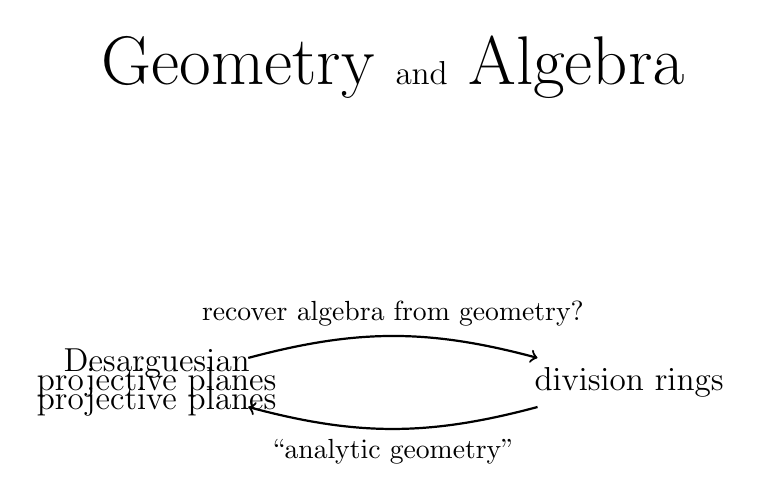
\begin{tikzpicture}
      \node (title) at (0,0) {\Huge Geometry {\large and} Algebra};

      \pause
      \alt<6->{
        \node (geometry) at (-3,-4) {\large \parbox{\widthof{\large
              projective planes}}{\begin{center}Desarguesian \\
            projective planes\end{center}}};
      }{
        \node (geometry) at (-3,-4) {\large projective planes};
      }
      
      \pause
      \node (algebra) at (3,-4) {\large division rings};

      \pause
      \draw[thick,->] (algebra) edge[in=-15,out=195] node[anchor=north]
      {``analytic geometry''} (geometry);
      
      \pause
      \draw[thick,->] (geometry) edge[in=165,out=15]
      node[anchor=south] {recover algebra from geometry?} (algebra);

    \end{tikzpicture}
  \end{center}
  \vfill
\end{frame}

%%%%%%%%%%%%%%%%%%%%%%%%%%%%%%%%%%%%%%%%%%%%%%%%%%%%%%%%%%%%%%%%
% analytic geometry
\begin{frame}
  \frametitle{Analytic geometry}

  \vfill
  \begin{center}
    \begin{tikzpicture}[scale=0.65]
      \coordinate (origin) at (0,0);
      \coordinate (x) at (10,0);
      \coordinate (y) at (0,10);

      \draw[->] ($ (origin)!-.1!(x) $) -- ($ (origin)!1.1!(x) $);
      \draw[->] ($ (origin)!-.1!(y) $) -- ($ (origin)!1.1!(y) $);

      \foreach \x in {1,...,10}
      \draw (\x,2pt) -- (\x,-5pt);
      \foreach \x in {1,...,10}
      \draw (2pt,\x) -- (-5pt,\x);
      
      \pause
      \fill (5,2) circle (6pt) node[anchor=south] {(5,2)};

      \pause
      \fill (7,6) circle (6pt) node[anchor=south] {(7,6)};

      \pause
      \fill (2,8) circle (6pt) node[anchor=south] {(2,8)};

    \end{tikzpicture}
  \end{center}
  \vfill

\end{frame}

\againframe<4-5>{overview}

%%%%%%%%%%%%%%%%%%%%%%%%%%%%%%%%%%%%%%%%%%%%%%%%%%%%%%%%%%%%%%%%
% analytic geometry
\begin{frame}
  \frametitle{Recover algebra from geometry?}

  \vfill
  \begin{center}
    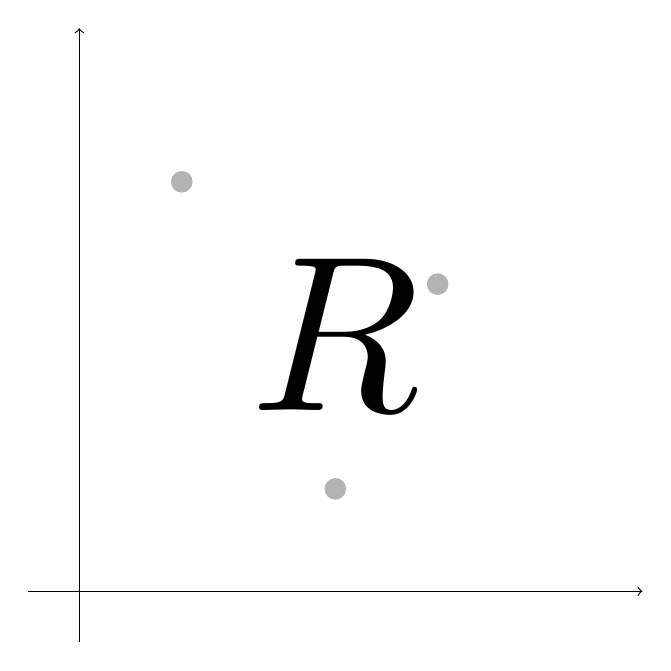
\begin{tikzpicture}[scale=0.65]
      \coordinate (origin) at (0,0);
      \coordinate (x) at (10,0);
      \coordinate (y) at (0,10);

      \draw[->] ($ (origin)!-.1!(x) $) -- ($ (origin)!1.1!(x) $);
      \draw[->] ($ (origin)!-.1!(y) $) -- ($ (origin)!1.1!(y) $);

      \pause
      \fill (5,2) circle (6pt);
      \fill (7,6) circle (6pt);
      \fill (2,8) circle (6pt);
      
      \pause
      \fill[color=white,opacity=0.7] (1,1) rectangle (10,10);
      \node (R) at (5,5) {\scalebox{8}{$\R$}};

    \end{tikzpicture}
  \end{center}
  \vfill

\end{frame}

\againframe<5>{overview}

\setbackgroundpicture{Railroad-Tracks-Perspective.jpg}
\begin{frame}[nofills,label=what-is-plane]
  \color{black}\Large\textbf{\scalebox{1.2}{What is a projective plane?}}
  \pause
  \vfill
  \vspace{0.5in}
  \color{white}\huge
  \begin{center}
  \textbf{Parallel lines} \\
  \textbf{meet at infinity}
  \end{center}
\end{frame}
\clearbackgroundpicture

%%%%%%%%%%%%%%%%%%%%%%%%%%%%%%%%%%%%%%%%%%%%%%%%%%%%%%%%%%%%%%%%
% axiomatic definition of projective plane
\begin{frame}
  \begin{definition}
   A \textbf{projective plane} consists of \\
   \quad a set of lines and a set of points, and \\
   \quad a relation (``incidence'') between points and lines, \\
   so that
   \begin{itemize}
   \item For any two distinct points, \\
     there exists a unique line incident with both.
   \item For any two distinct lines, \\
     there exists a unique point incident with both.
   \end{itemize}
  \end{definition}

  \pause

  There are four points such that \\
  \quad no line is incident with more than two of them \\
  \pause\quad (i.e., there's a quadrilateral).

\end{frame}

%%%%%%%%%%%%%%%%%%%%%%%%%%%%%%%%%%%%%%%%%%%%%%%%%%%%%%%%%%%%%%%%
% Fano plane, first example
\begin{frame}[label=fano]
  \begin{center}
  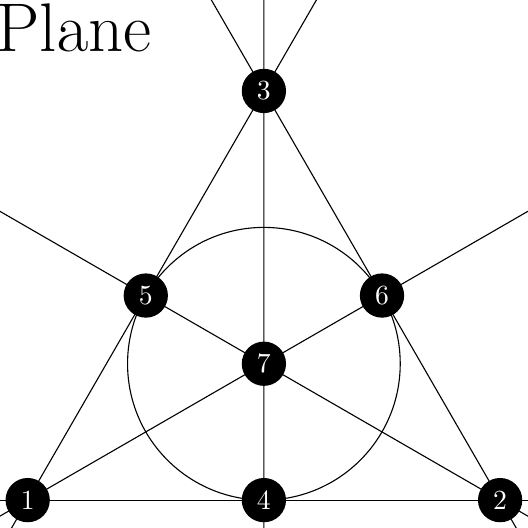
\begin{tikzpicture}
    \useasboundingbox (0,0) rectangle (6,6);

    \coordinate (A) at (0,0); 
    \coordinate (B) at (6,0);
    \coordinate (C) at ($ (A)!1!60:(B) $); 

    \coordinate (AB) at ($ (A)!.5!(B) $); 
    \coordinate (AC) at ($ (A)!.5!(C) $); 
    \coordinate (BC) at ($ (B)!.5!(C) $); 
    \coordinate (ABC) at ($ (A)!2.0/3.0!(BC) $); 

    \fill (A) circle (8pt);
    \fill (B) circle (8pt);
    \fill (C) circle (8pt);
    \fill (AB) circle (8pt);
    \fill (AC) circle (8pt);
    \fill (BC) circle (8pt);
    \fill (ABC) circle (8pt);

    \pause
    \draw ($ (A)!-15!(B) $) -- ($ (A)!15!(B) $);

    \pause
    \draw ($ (C)!-15!(B) $) -- ($ (C)!15!(B) $);

    \pause
    \draw ($ (A)!-15!(C) $) -- ($ (A)!15!(C) $);

    \pause
    \draw ($ (A)!-15!(ABC) $) -- ($ (A)!15!(ABC) $);
    \pause
    \draw ($ (B)!-15!(ABC) $) -- ($ (B)!15!(ABC) $);
    \pause
    \draw ($ (C)!-15!(ABC) $) -- ($ (C)!15!(ABC) $);

    \pause
    \node[draw,circle through=(BC)] at (ABC) {};

    \pause
    \draw (-0.4,6) node {\Huge Fano Plane};

    \pause
    \draw  (A) node[color=white] {$1$};
    \draw  (B) node[color=white] {$2$};
    \draw  (C) node[color=white] {$3$};
    \draw  (AB) node[color=white] {$4$};
    \draw  (AC) node[color=white] {$5$};
    \draw  (BC) node[color=white] {$6$};
    \draw  (ABC) node[color=white] {$7$};
    
    \pause
    \draw (3,-0.9) node[fill=white,fill opacity=0.75,text opacity=1]
    {points $= \{ 1, 2, 3, 4, 5, 6, 7 \}$};

    \pause
    \draw (3,-1.7) node[fill=white,fill opacity=0.75,text opacity=1] {lines $= \{ 124,135,236, 257, 167, 347, 456\}$};
    
  \end{tikzpicture}
\end{center}
\end{frame}

%%%%%%%%%%%%%%%%%%%%%%%%%%%%%%%%%%%%%%%%%%%%%%%%%%%%%%%%%%%%%%%%
\begin{frame}
  \frametitle{Seven points is not an accident}

  \begin{theorem}
    If there are finitely many points, then \\
    \quad there are $N^2 + N + 1$ points, \\
    \quad there are $N^2 + N + 1$ lines, \\
    \quad with $N+1$ points on each line, and \\
    \quad with $N+1$ lines through each point. \\    
  \end{theorem}
  \pause
  
    \begin{center}
    \begin{columns}
      \begin{column}{0.4\textwidth}
        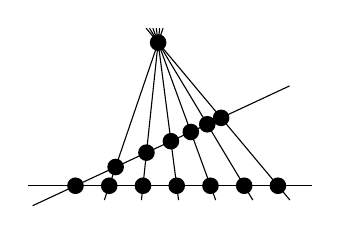
\begin{tikzpicture}[scale=3]
          \draw[name path=x axis] (0:-0.2) -- (0:1);
          \draw[name path=y axis] (25:-0.2) -- (25:1);

          \fill (0,0) circle (1pt);
          \pause
          \coordinate (c) at (60:0.7);
          \fill (c) circle (1pt);
          \pause
          \foreach \x in {1,...,6}
          \fill (0:{\x/7}) circle (1pt);
          \pause
          \foreach \x in {1,...,6} {
            \draw[name path=line] ($ (c)!-.1!(0:{\x/7}) $) -- ($ (c)!1.1!(0:{\x/7}) $);
            \path [name intersections={of=line and y axis, by=point}] ;
            \fill (point) circle (1pt);
          }

        \end{tikzpicture}
      \end{column}
      \begin{column}{0.4\textwidth}
        \uncover<6->{%
          Any two lines have the same number of points.\hfill\uncover<7->{\qed}
        }
      \end{column}
    \end{columns}
    \end{center}

\end{frame}

%%%%%%%%%%%%%%%%%%%%%%%%%%%%%%%%%%%%%%%%%%%%%%%%%%%%%%%%%%%%%%%%
% definition of division ring
\begin{frame}[label=definition-division-ring]
  \begin{definition}
    A \uncover<2->{\textbf{division ring}} \textcolor{gray}{\uncover<2->{(``skew} \alt<1>{\textcolor{black}{field}}{field}\uncover<2->{'')}} is a set $R$ \\
    \quad with two operations $+$ and $\times$ \\
    \quad so that $(R,+)$ is an abelian group with identity 0\\
    \quad and $(R \setminus \{0\},\times)$ is a\uncover<1>{n abelian} group \\
    \quad\quad so that $\times$ distributes over $+$.
  \end{definition}

  \vfill
  \uncover<3->{
  \textbf{Warning:} Multiplication in a division ring \\
  \quad does not necessarily commute!}
\end{frame}

%%%%%%%%%%%%%%%%%%%%%%%%%%%%%%%%%%%%%%%%%%%%%%%%%%%%%%%%%%%%%%%%
% build projective plane from division ring
\begin{frame}
  \frametitle{From rings to planes}

  $R$ be a division ring.

  \vfill\pause

  $P^2(R)$ is a projective plane, in which
  \begin{description}
  \item[``points''] are lines in $R^3$,
  \item[``lines''] are planes in $R^3$.
  \end{description}

  \vfill\pause

  Check that incidence properties are satisfied.

\end{frame}

\begin{frame}
  \frametitle{Coordinates}

  \vfill

  Coordinates for points in $P^2(R)$ are \\
  \quad $[x:y:z]$ for $x, y, z \in R$, \\
  \quad where $(x,y,z) \neq (0,0,0)$. \\
  \vspace{3ex}
  where $[x:y:z] = [\lambda x:\lambda y:\lambda z]$, \\
  \quad for $\lambda \in R$.

  \vfill

\end{frame}

%%%%%%%%%%%%%%%%%%%%%%%%%%%%%%%%%%%%%%%%%%%%%%%%%%%%%%%%%%%%%%%%
% example of building a projective plane
\begin{frame}
  $\mathbb{F}_2 = \{ 0, 1 \}$.

  \vfill\pause

  ${\mathbb{F}_2}^3 = \{ 000, 001, 010, 011, 100, 101, 110, 111 \}$

  \vfill\pause
  7 lines in ${\mathbb{F}_2}^3$,\pause\ e.g., $[0:0:1]$.

  \vfill\pause
  7 planes in ${\mathbb{F}_2}^3$. \\
  \quad $\{ 000, 001, 010, 011 \}$, $\{ 000, 010, 100, 110 \}$, \\
  \quad $\{ 000, 100, 001, 101 \}$, $\{ 000, 100, 011, 111 \}$, \\
  \quad $\{ 000, 010, 101, 111 \}$, $\{ 000, 001, 110, 111 \}$, \\
  \quad $\{ 000, 101, 110, 011 \}$.

  \vfill\pause

  So $P^2(\mathbb{F}_2)$ is the \textbf{Fano plane}.

\end{frame}

\againframe<10>{fano}

\begin{frame}
  $\mathbb{F}_3 = \{ 0, 1, 2 \}$.

  \vfill\pause

  \begin{align*}
  {\mathbb{F}_3}^3 = \{
  & 000, 001, 002,
  010, 011, 012,
  020, 021, 022, \\
  & 100, 101, 102,
  110, 111, 112,
  120, 121, 122, \\
  & 200, 201, 202,
  210, 211, 212,
  220, 221, 222 \}.
  \end{align*}

  \vfill\pause
  For example, a line in ${\mathbb{F}_3}^3$ is
  $$
  \{ 000, 012, 021 \}.
  $$
  and a plane in ${\mathbb{F}_3}^3$ is
  $$
  \{ 000, 012, 021, 100, 200, 112, 212, 121, 221 \}.
  $$
  \pause
  There are 13 lines and 13 planes in ${\mathbb{F}_3}^3$.

\end{frame}

\begin{frame}
\scriptsize 
  \begin{align*}
    \mbox{lines} = & \{ 000,001,002 \}, \{ 000,010,020 \}, \{ 000,011,022 \}, \{ 000,012,021 \},\\
    & \{ 000,100,200 \}, \{ 000,101,202 \}, \{ 000,102,201 \}, \{ 000,110,220 \},\\
    & \{ 000,111,222 \}, \{ 000,112,221 \}, \{ 000,120,210 \}, \{ 000,121,212 \},\\
    & \{ 000,122,211 \},
  \end{align*}

  \begin{align*}
    \mbox{planes} = & \{ 000,001,002,010,011,012,020,021,022 \}\\
    & \{ 000,010,020,100,110,120,200,210,220 \}\\
    & \{ 000,012,021,101,110,122,202,211,220 \}\\
    & \{ 000,012,021,102,111,120,201,210,222 \}\\
    & \{ 000,001,002,110,111,112,220,221,222 \}\\
    & \{ 000,011,022,101,112,120,202,210,221 \}\\
    & \{ 000,011,022,102,110,121,201,212,220 \}\\
    & \{ 000,012,021,100,112,121,200,212,221 \}\\
    & \{ 000,010,020,102,112,122,201,211,221 \}\\
    & \{ 000,010,020,101,111,121,202,212,222 \}\\
    & \{ 000,011,022,100,111,122,200,211,222 \}\\
    & \{ 000,001,002,100,101,102,200,201,202 \}\\
    & \{ 000,001,002,120,121,122,210,211,212 \}
  \end{align*}
    
\end{frame}

\begin{frame}
  \begin{columns}
    \begin{column}{0.5\textwidth}
 \begin{align*}
   \mbox{13 ``points''} =& \{1, 2, 3, \ldots, 13 \} \\
   \mbox{13 ``lines''} =& \{ \{ 1,2,3,4 \}, \\
   & \{ 2,5,8,11 \}, \\
   & \{ 4,6,8,13 \},  \\
   & \{ 4,7,9,11 \}, \\
   & \{ 1,8,9,10 \}, \\
   & \{ 3,6,10,11 \}, \\ 
   &   \{ 3,7,8,12 \},\\
   & \{ 4,5,10,12 \},\\
   & \{ 2,7,10,13 \},  \{ 2,6,9,12 \}, \\
   &  \{ 3,5,9,13 \},  \{ 1,5,6,7 \}, \\
   &  \{ 1,11,12,13 \} \}
 \end{align*}
 \end{column}
    \begin{column}{0.5\textwidth}
      \null\hspace{-1in}
  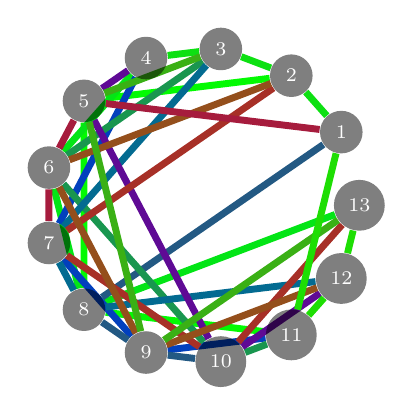
\begin{tikzpicture}[scale=2]
\node[fill=white,circle] (1) at (27.6923076923077:1) {\textcolor{white}{\scriptsize$1$}};
\node[fill=white,circle] (2) at (55.3846153846154:1) {\textcolor{white}{\scriptsize$2$}};
\node[fill=white,circle] (3) at (83.0769230769231:1) {\textcolor{white}{\scriptsize$3$}};
\node[fill=white,circle] (4) at (110.769230769231:1) {\textcolor{white}{\scriptsize$4$}};
\node[fill=white,circle] (5) at (138.461538461538:1) {\textcolor{white}{\scriptsize$5$}};
\node[fill=white,circle] (6) at (166.153846153846:1) {\textcolor{white}{\scriptsize$6$}};
\node[fill=white,circle] (7) at (193.846153846154:1) {\textcolor{white}{\scriptsize$7$}};
\node[fill=white,circle] (8) at (221.538461538462:1) {\textcolor{white}{\scriptsize$8$}};
\node[fill=white,circle] (9) at (249.230769230769:1) {\textcolor{white}{\scriptsize$9$}};
\node[fill=white,circle] (10) at (276.923076923077:1) {\textcolor{white}{\scriptsize$10$}};
\node[fill=white,circle] (11) at (304.615384615385:1) {\textcolor{white}{\scriptsize$11$}};
\node[fill=white,circle] (12) at (332.307692307692:1) {\textcolor{white}{\scriptsize$12$}};
\node[fill=white,circle] (13) at (360.0:1) {\textcolor{white}{\scriptsize$13$}};

\draw[line width=2.5pt,color=red!41!blue!12!green] (1) to (2) to (3) to (4);
\draw[line width=2.5pt,color=red!60!blue!2!green] (2) to (5) to (8) to (11);
\draw[line width=2.5pt,color=red!12!blue!10!green] (4) to (6) to (8) to (13);
\draw[line width=2.5pt,color=red!1!blue!75!green] (4) to (7) to (9) to (11);
\draw[line width=2.5pt,color=red!21!blue!65!green] (1) to (8) to (9) to (10);
\draw[line width=2.5pt,color=red!24!blue!41!green] (3) to (6) to (10) to (11);
\draw[line width=2.5pt,color=red!2!blue!58!green] (3) to (7) to (8) to (12);
\draw[line width=2.5pt,color=red!39!blue!96!green] (4) to (5) to (10) to (12);
\draw[line width=2.5pt,color=red!81!blue!81!green] (2) to (7) to (10) to (13);
\draw[line width=2.5pt,color=red!84!blue!69!green] (2) to (6) to (9) to (12);
\draw[line width=2.5pt,color=red!74!blue!31!green] (3) to (5) to (9) to (13);
\draw[line width=2.5pt,color=red!73!blue!89!green] (1) to (5) to (6) to (7);
\draw[line width=2.5pt,color=red!89!blue!13!green] (1) to (11) to (12) to (13);

\node[fill=black, fill opacity=0.5,text opacity=1,circle] (1) at (27.6923076923077:1) {\textcolor{white}{\scriptsize$1$}};
\node[fill=black, fill opacity=0.5,text opacity=1,circle] (2) at (55.3846153846154:1) {\textcolor{white}{\scriptsize$2$}};
\node[fill=black, fill opacity=0.5,text opacity=1,circle] (3) at (83.0769230769231:1) {\textcolor{white}{\scriptsize$3$}};
\node[fill=black, fill opacity=0.5,text opacity=1,circle] (4) at (110.769230769231:1) {\textcolor{white}{\scriptsize$4$}};
\node[fill=black, fill opacity=0.5,text opacity=1,circle] (5) at (138.461538461538:1) {\textcolor{white}{\scriptsize$5$}};
\node[fill=black, fill opacity=0.5,text opacity=1,circle] (6) at (166.153846153846:1) {\textcolor{white}{\scriptsize$6$}};
\node[fill=black, fill opacity=0.5,text opacity=1,circle] (7) at (193.846153846154:1) {\textcolor{white}{\scriptsize$7$}};
\node[fill=black, fill opacity=0.5,text opacity=1,circle] (8) at (221.538461538462:1) {\textcolor{white}{\scriptsize$8$}};
\node[fill=black, fill opacity=0.5,text opacity=1,circle] (9) at (249.230769230769:1) {\textcolor{white}{\scriptsize$9$}};
\node[fill=black, fill opacity=0.5,text opacity=1,circle] (10) at (276.923076923077:1) {\textcolor{white}{\scriptsize$10$}};
\node[fill=black, fill opacity=0.5,text opacity=1,circle] (11) at (304.615384615385:1) {\textcolor{white}{\scriptsize$11$}};
\node[fill=black, fill opacity=0.5,text opacity=1,circle] (12) at (332.307692307692:1) {\textcolor{white}{\scriptsize$12$}};
\node[fill=black, fill opacity=0.5,text opacity=1,circle] (13) at (360.0:1) {\textcolor{white}{\scriptsize$13$}};

\end{tikzpicture}
\end{column}
\end{columns}
  
\end{frame}

\begin{frame}[label=real-projective-plane]
  \frametitle{Real projective plane}

  \begin{columns}
    \begin{column}{0.5\textwidth}
      $P^2(\mathbb{R}) = \mathbb{R}P^2$

      \vspace{3ex}
      \uncover<2->{Points in $\mathbb{R}P^2$ are\\
        \quad lines in $\R^3$.}

      \vspace{3ex}
      \uncover<3->{Lines in $\mathbb{R}P^2$ are \\
        \quad planes in $\R^3$.}

      \vspace{3ex}
      \uncover<4->{$\dim \mathbb{R}P^2 = 2$.}
    \end{column}
    \begin{column}{0.5\textwidth}
      \uncover<5->{
        \begin{tikzpicture} % "THE GLOBE" showcase
          \useasboundingbox (-2,-2) rectangle (2,2);

          \def\R{2.5} % sphere radius
          \def\angEl{25} % elevation angle
          \def\angAz{105} % azimuth angle
          \filldraw[ball color=white] (0,0) circle (\R);
          \foreach \t in {-80,-60,...,80} { \DrawLatitudeCircle[\R]{\t} }
          \foreach \t in {-5,-35,...,-175} { \DrawLongitudeCircle[\R]{\t} }

          \uncover<6->{
            \begin{scope}
              \def\angPhi{-56} % longitude of point P
              \def\angBeta{45} % latitude of point P
              \only<7->{
                \def\angPhi{-46} % longitude of point P
                \def\angBeta{35} % latitude of point P
              }
              \only<8->{
                \def\angPhi{-36} % longitude of point P
                \def\angBeta{25} % latitude of point P
              }
              \only<9->{
                \def\angPhi{-26} % longitude of point P
                \def\angBeta{15} % latitude of point P
              }
              \only<10->{
                \def\angPhi{-16} % longitude of point P
                \def\angBeta{5} % latitude of point P
              }
              \only<11->{
                \def\angPhi{-6} % longitude of point P
                \def\angBeta{-5} % latitude of point P
              }
              \only<12->{
                \def\angPhi{4} % longitude of point P
                \def\angBeta{-15} % latitude of point P
              }
              \only<13->{
                \def\angPhi{14} % longitude of point P
                \def\angBeta{-25} % latitude of point P
              }
              \only<14->{
                \def\angPhi{24} % longitude of point P
                \def\angBeta{-35} % latitude of point P
              }
              \only<15->{
                \def\angPhi{34} % longitude of point P
                \def\angBeta{-45} % latitude of point P
              }
              \only<16->{
                \def\angPhi{44} % longitude of point P
                \def\angBeta{-55} % latitude of point P
              }
              \only<17->{
                \def\angPhi{54} % longitude of point P
                \def\angBeta{-65} % latitude of point P
              }
              \only<18->{
                \def\angPhi{64} % longitude of point P
                \def\angBeta{-75} % latitude of point P
              }
              \only<19->{
                \def\angPhi{74} % longitude of point P
                \def\angBeta{-85} % latitude of point P
              }
              \only<20->{
                \def\angPhi{264} % longitude of point P
                \def\angBeta{85} % latitude of point P
              }
              \only<21->{
                \def\angPhi{274} % longitude of point P
                \def\angBeta{75} % latitude of point P
              }
              \only<22->{
                \def\angPhi{284} % longitude of point P
                \def\angBeta{65} % latitude of point P
              }
              \only<23->{
                \def\angPhi{294} % longitude of point P
                \def\angBeta{55} % latitude of point P
              }


              %% working planes
              
              \pgfmathsetmacro\H{\R*cos(\angEl)} % distance to north pole
              \tikzset{xyplane/.estyle={cm={cos(\angAz),sin(\angAz)*sin(\angEl),-sin(\angAz),
                    cos(\angAz)*sin(\angEl),(0,-\H)}}}
              \LongitudePlane[xzplane]{\angEl}{\angAz}
              \LongitudePlane[pzplane]{\angEl}{\angPhi}
              \LatitudePlane[equator]{\angEl}{0}
              
              %% draw xyplane and sphere
              
              % \draw[xyplane] (-2*\R,-2*\R) rectangle (2.2*\R,2.8*\R);
              % \fill[ball color=white] (0,0) circle (\R); % 3D lighting effect
              % \draw (0,0) circle (\R);
              
              %% characteristic points

              \coordinate (O) at (0,0);
              \coordinate (N) at (0,\H);
              \coordinate (S) at (0,-\H);
              \path[pzplane] (\angBeta:\R) coordinate (P);
              \path[pzplane] (\R,0) coordinate (PE);
              \path[xzplane] (\R,0) coordinate (XE);
              \path (PE) ++(0,-\H) coordinate (Paux); % to aid Phat calculation
              \coordinate (Phat) at (intersection cs: first line={(N)--(P)},
              second line={(S)--(Paux)});
              
              \fill (P) circle (3pt);
            \end{scope}
            \begin{scope}
              \def\angPhi{124} % longitude of point P
              \def\angBeta{-45} % latitude of point P
              \only<7->{
                \def\angPhi{134} % longitude of point P
                \def\angBeta{-35} % latitude of point P
              }
              \only<8->{
                \def\angPhi{144} % longitude of point P
                \def\angBeta{-25} % latitude of point P
              }
              \only<9->{
                \def\angPhi{154} % longitude of point P
                \def\angBeta{-15} % latitude of point P
              }
              \only<10->{
                \def\angPhi{164} % longitude of point P
                \def\angBeta{-5} % latitude of point P
              }
              \only<11->{
                \def\angPhi{174} % longitude of point P
                \def\angBeta{5} % latitude of point P
              }
              \only<12->{
                \def\angPhi{184} % longitude of point P
                \def\angBeta{15} % latitude of point P
              }
              \only<13->{
                \def\angPhi{194} % longitude of point P
                \def\angBeta{25} % latitude of point P
              }
              \only<14->{
                \def\angPhi{204} % longitude of point P
                \def\angBeta{35} % latitude of point P
              }
              \only<15->{
                \def\angPhi{214} % longitude of point P
                \def\angBeta{45} % latitude of point P
              }
              \only<16->{
                \def\angPhi{224} % longitude of point P
                \def\angBeta{55} % latitude of point P
              }
              \only<17->{
                \def\angPhi{234} % longitude of point P
                \def\angBeta{65} % latitude of point P
              }
              \only<18->{
                \def\angPhi{244} % longitude of point P
                \def\angBeta{75} % latitude of point P
              }
              \only<19->{
                \def\angPhi{254} % longitude of point P
                \def\angBeta{85} % latitude of point P
              }
              \only<20->{
                \def\angPhi{84} % longitude of point P
                \def\angBeta{-85} % latitude of point P
              }
              \only<21->{
                \def\angPhi{94} % longitude of point P
                \def\angBeta{-75} % latitude of point P
              }
              \only<22->{
                \def\angPhi{104} % longitude of point P
                \def\angBeta{-65} % latitude of point P
              }
              \only<23->{
                \def\angPhi{114} % longitude of point P
                \def\angBeta{-55} % latitude of point P
              }

              %% working planes
              
              \pgfmathsetmacro\H{\R*cos(\angEl)} % distance to north pole
              \tikzset{xyplane/.estyle={cm={cos(\angAz),sin(\angAz)*sin(\angEl),-sin(\angAz),
                    cos(\angAz)*sin(\angEl),(0,-\H)}}}
              \LongitudePlane[xzplane]{\angEl}{\angAz}
              \LongitudePlane[pzplane]{\angEl}{\angPhi}
              \LatitudePlane[equator]{\angEl}{0}
              
              %% draw xyplane and sphere
              
              % \draw[xyplane] (-2*\R,-2*\R) rectangle (2.2*\R,2.8*\R);
              % \fill[ball color=white] (0,0) circle (\R); % 3D lighting effect
              % \draw (0,0) circle (\R);
              
              %% characteristic points

              \coordinate (O) at (0,0);
              \coordinate (N) at (0,\H);
              \coordinate (S) at (0,-\H);
              \path[pzplane] (\angBeta:\R) coordinate (Q);
              \path[pzplane] (\R,0) coordinate (PE);
              \path[xzplane] (\R,0) coordinate (XE);
              \path (PE) ++(0,-\H) coordinate (Paux); % to aid Phat calculation
              \coordinate (Phat) at (intersection cs: first line={(N)--(Q)},
              second line={(S)--(Paux)});
              
              \fill (Q) circle (3pt);

              \draw[line width=1.5pt] (P) -- (Q);
              \draw[line width=0.5pt,->] ($ (P)!1!(Q) $) -- ($ (P)!2!(Q) $);
              \draw[line width=0.5pt,->] ($ (P)!0!(Q) $) -- ($ (P)!-1!(Q) $);
            \end{scope}
          }

        \end{tikzpicture}
      }
    \end{column}
  \end{columns}
  \uncover<24>{.}
\end{frame}

\begin{frame}[label=identification-polygon]

  \begin{center}
    \begin{tikzpicture}[scale=6]
      \draw (0,0) rectangle (1,1);
      \draw[
      decoration={markings,mark=at position 1 with {\arrow[scale=4]{>}}},
      postaction={decorate},
      shorten >=0.4pt
      ]
      (0,0) -- (0,0.55);
      
      \draw[
      decoration={markings,mark=at position 1 with {\arrow[scale=4]{>}}},
      postaction={decorate},
      shorten >=0.4pt
      ]
      (1,1) -- (1,0.45);
      
      \draw[
      decoration={markings,mark=at position 1 with {\arrow[scale=4]{>}}},
      postaction={decorate},
      shorten >=0.4pt
      ]
      (0,0) -- (0.50,0);
      \draw[
      decoration={markings,mark=at position 1 with {\arrow[scale=4]{>}}},
      postaction={decorate},
      shorten >=0.4pt
      ]
      (0,0) -- (0.55,0);
      \draw[
      decoration={markings,mark=at position 1 with {\arrow[scale=4]{>}}},
      postaction={decorate},
      shorten >=0.4pt
      ]
      (1,1) -- (0.50,1);
      \draw[
      decoration={markings,mark=at position 1 with {\arrow[scale=4]{>}}},
      postaction={decorate},
      shorten >=0.4pt
      ]
      (1,1) -- (0.45,1);
      
    \end{tikzpicture}
  \end{center}
  
\end{frame}

%%%%%%%%%%%%%%%%%%%%%%%%%%%%%%%%%%%%%%%%%%%%%%%%%%%%%%%%%%%%%%%%
\begin{frame}
  \frametitle{Complex projective plane}

  %BADBAD could include a picture here

  \vfill
  \begin{center}
    \scalebox{6}{$\mathbb{C}P^2$}
  \end{center}
  \vfill
  
  $\dim_{\mathbb{R}} \mathbb{C}P^2 = 4$.
\end{frame}


%%%%%%%%%%%%%%%%%%%%%%%%%%%%%%%%%%%%%%%%%%%%%%%%%%%%%%%%%%%%%%%%
% main question
\begin{frame}[label=main-question]
  \begin{center}
    \large
  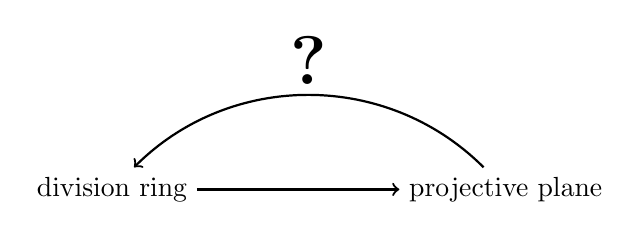
\begin{tikzpicture}
    \node (division) at (0,0) {division ring};
    \node (projective) at (5,0) {projective plane};
    \only<2->{
      \draw [thick,->] (division) -- (projective);
    }
    \uncover<5->{
      \draw [thick,->] (projective) edge[out=135,in=45] node[above] {\Huge\textbf{?}} (division);
    }
    
  \end{tikzpicture}
  \end{center}
  \uncover<3->{What about going the other way?}

  \vfill

  \Large

  \uncover<4->{Given a projective plane, \\
    \quad can I recover a division ring?}

  \vfill
\end{frame}

\againframe<4-5>{overview}

%%%%%%%%%%%%%%%%%%%%%%%%%%%%%%%%%%%%%%%%%%%%%%%%%%%%%%%%%%%%%%%%
\begin{frame}[label=how-to-add]
\frametitle{How to add}

\begin{center}
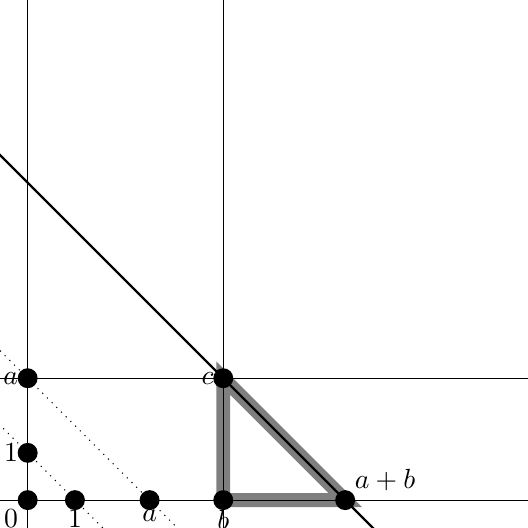
\begin{tikzpicture}[scale=0.6]
  \useasboundingbox (0,0) rectangle (10,10);
  \coordinate (origin) at (0,0);
  \coordinate (x) at (10,0);
  \coordinate (y) at (0,10);

  \draw[->] ($ (origin)!-.1!(x) $) -- ($ (origin)!1.1!(x) $);
  \draw[->] ($ (origin)!-.1!(y) $) -- ($ (origin)!1.1!(y) $);

  \coordinate (one) at (1,0);
  \coordinate (one') at (0,1);

  \pause
  \fill (one) circle (6pt) node[anchor=north] {1};
  \fill (origin) circle (6pt) node[anchor=north east] {0};

  \pause
  \fill (one') circle (6pt) node[anchor=east] {1};

  \pause
  \draw[dotted] ($ (one)!-15!(one') $) -- ($ (one)!15!(one') $);

  \pause
  \coordinate (a) at (2.58,0);
  \coordinate (b) at (4.14,0);
  \coordinate (ab) at (6.72,0);
  \coordinate (a') at (0,2.58);
  \coordinate (b') at (0,4.14);

  \fill (a) circle (6pt) node[anchor=north] {$a$};
  \fill (b) circle (6pt) node[anchor=north] {$b$};

  \pause
  \draw[dotted] ($ (a)!-15!(a') $) -- ($ (a)!15!(a') $);
%  \draw[dotted] ($ (b)!-15!(b') $) -- ($ (b)!15!(b') $);

  \pause
  \fill (a') circle (6pt) node[anchor=east] {$a$};
%  \fill (b') circle (6pt) node[anchor=east] {$b$};

  \pause
  \draw (a') ++ (-20,0) -- ++ (40,0);
  \pause
  \draw (b) ++ (0,-20) -- ++ (0,40);

  \pause
  \coordinate (c) at (4.14,2.58);
  \fill (c) circle (6pt) node[anchor=east] {$c$};

  \pause
  \draw[thick] ($ (c)!-15!(ab) $) -- ($ (c)!15!(ab) $);

  \pause
  \fill (ab) circle (6pt) node[anchor=south west] {$a+b$};

  \pause
  \draw[line width=5pt,opacity=0.5] (c) -- (b) -- (ab) -- cycle;

\end{tikzpicture}
\end{center}

\end{frame}

\begin{frame}[label=plan-of-attack]
\frametitle{How to add (in projective plane)}

\textcolor{blue}{Theorem in Euclidean plane} \\
\quad that a certain construction on $(a,0)$ and $(b,0)$ \\
\quad results in $(a+b,0)$.

\vfill
\pause

\textcolor{blue}{Definition for a projective plane} \\
\quad that $a$ ``plus'' $b$ results from \\
\quad that same construction.

\vfill
\pause

Elements of division ring will be \\
\quad all but one of the \\
\quad points on a chosen line.

\end{frame}

%%%%%%%%%%%%%%%%%%%%%%%%%%%%%%%%%%%%%%%%%%%%%%%%%%%%%%%%%%%%%%%%
\begin{frame}<1-17>[label=adding]
\frametitle{How to add (in projective plane)}

\begin{center}
\begin{tikzpicture}[scale=0.6]
  \useasboundingbox (-2,0) rectangle (10,10);
  \coordinate (origin) at (0,0);
  \coordinate (x) at (10,0);
  \coordinate (y) at (4,10);

  \draw[->, name path=x axis] ($ (origin)!-.1!(x) $) -- ($ (origin)!1.1!(x) $);
  \draw[->, name path=y axis] ($ (origin)!-.1!(y) $) -- ($ (origin)!1.1!(y) $);

  \coordinate (one) at (1,0);
  \coordinate (one') at ($ (origin)!0.1!(y) $);

  \draw[name path=circle at infinity] (origin) circle (4in);

  \path [name intersections={of=x axis and circle at infinity, by=x infinity}] ;
  \path [name intersections={of=y axis and circle at infinity, by=y infinity}] ;

  \pause
  \fill (one) circle (6pt) node[anchor=north] {1};
  \fill (origin) circle (6pt) node[anchor=north east] {0};

  \pause
  \fill (one') circle (6pt) node[anchor=east] {1};

  \pause
  \draw[dotted,name path=one line] ($ (one)!-15!(one') $) -- ($ (one)!15!(one') $);

  \path [name intersections={of=one line and circle at infinity, by=one-infinity}] ;
  \fill (one-infinity) circle (6pt) node[anchor=east] {$1_\infty$};

  \pause
  \coordinate (a) at (2.58,0);
  \coordinate (b) at (4.14,0);

  \fill (a) circle (6pt) node[anchor=north east] {$a$};
  \fill (b) circle (6pt) node[anchor=north east] {$b$};

  \pause
  \draw[dotted,name path=a one line] ($ (a)!-15!(one-infinity) $) -- ($ (a)!15!(one-infinity) $);
  \path [name intersections={of=a one line and y axis, by=a'}] ;
  \fill (a') circle (6pt) node[anchor=east] {$a'$};

  \pause
  \draw[name path=a x infinity] ($ (a')!-15!(x infinity) $) -- ($ (a')!15!(x infinity) $);
  \pause
  \draw[name path=b y infinity] ($ (b)!-15!(y infinity) $) -- ($ (b)!15!(y infinity) $);

  \pause
  \path [name intersections={of=a x infinity and b y infinity, by=c}] ;
  \fill (c) circle (6pt) node[anchor=south west] {$c$};

  \pause
  \draw[thick,name path=c one line] ($ (c)!-15!(one-infinity) $) -- ($ (c)!15!(one-infinity) $);

  \pause
  \path [name intersections={of=c one line and x axis, by=ab}] ;
  \fill (ab) circle (6pt) node[anchor=north] {$a+b$};

  \pause
  \draw[dotted,name path=b one line] ($ (b)!-15!(one-infinity) $) -- ($ (b)!15!(one-infinity) $);
  \path [name intersections={of=b one line and y axis, by=b'}] ;
  \fill (b') circle (6pt) node[anchor=east] {$b'$};

  \pause
  \draw[name path=b x infinity] ($ (b')!-15!(x infinity) $) -- ($ (b')!15!(x infinity) $);
  \pause
  \draw[name path=a y infinity] ($ (a)!-15!(y infinity) $) -- ($ (a)!15!(y infinity) $);

  \pause
  \path [name intersections={of=a y infinity and b x infinity, by=c'}] ;
  \fill (c') circle (6pt) node[anchor=south west] {$c'$};

  \pause
  \draw[thick,name path=c' one line] ($ (c')!-15!(one-infinity) $) -- ($ (c')!15!(one-infinity) $);

  \pause
  \path [name intersections={of=c' one line and x axis, by=ba}] ;
  \fill (ba) circle (6pt) node[anchor=south] {$b+a$};

  \pause%18
  \only<18-22>{
    \path [draw,fill opacity=0.25,fill=red] (a') -- (b') -- (x infinity) -- cycle;
    \path [draw,fill opacity=0.25,fill=blue] (a) -- (b) -- (y infinity)
    -- cycle;
  }

  \pause%19
  \only<19>{
    \draw[line width=6pt,opacity=0.5] ($ (one-infinity)!-15!(a) $) -- ($ (one-infinity)!15!(a) $);
    \draw[line width=6pt,opacity=0.5] ($ (one-infinity)!-15!(b) $) -- ($ (one-infinity)!15!(b) $);
    \draw[line width=6pt,opacity=0.5] (origin) circle (4in);
  }

  \pause%20
  \only<20-22>{
    \draw[red,line width=6pt,opacity=.25] ($ (a)!-15!(b) $) -- ($ (a)!15!(b) $);
    \draw[red,line width=6pt,opacity=.25] ($ (a')!-15!(b') $) -- ($ (a')!15!(b') $);
    \draw[green,line width=6pt,opacity=.25] ($ (b')!-15!(x infinity) $) -- ($ (b')!15!(x infinity) $);
    \draw[green,line width=6pt,opacity=.25] ($ (b)!-15!(y infinity) $) -- ($ (b)!15!(y infinity) $);
    \draw[blue,line width=6pt,opacity=.25] ($ (a')!-15!(x infinity) $) -- ($ (a')!15!(x infinity) $);
    \draw[blue,line width=6pt,opacity=.25] ($ (a)!-15!(y infinity) $) -- ($ (a)!15!(y infinity) $);
  }

  \pause%21
  \path [name intersections={of=a y infinity and a x infinity, by=d}] ;
  \path [name intersections={of=b x infinity and b y infinity, by=d'}] ;

  \fill (d) circle (6pt) node[anchor=north east] {$d$};
  \fill (d') circle (6pt) node[anchor=south west] {$d'$};

  \pause%22
  \only<22-25>{
    \draw[line width=5pt,opacity=0.5] ($ (origin)!-10!(d) $) to
    (origin) to (d) to (d') to ($ (d)!10!(d') $);
  }

  \pause%23
  \draw[name path=ba' line] ($ (b)!-15!(a') $) -- ($ (b)!15!(a') $);
  \draw[name path=ab' line] ($ (a)!-15!(b') $) -- ($ (a)!15!(b') $);

  \only<23-26>{
    \path [draw,fill opacity=0.25,fill=red] (a) -- (b') -- (x
    infinity) -- cycle;
    \path [draw,fill opacity=0.25,fill=blue] (a') -- (b) -- (y infinity) --
    cycle;
    \path [name intersections={of=ab' line and ba' line, by=e}] ;
  }

  \pause%24
  \only<24>{
    \draw[line width=6pt,opacity=0.5] ($ (a)!-15!(a') $) -- ($ (a)!15!(a') $);
    \draw[line width=6pt,opacity=0.5] ($ (b')!-15!(b) $) -- ($ (b')!15!(b) $);
    \draw[line width=6pt,opacity=0.5] (origin) circle (4in);
  }

  \pause%25
  \only<25-26>{
    \draw[red,line width=6pt,opacity=.25] ($ (a)!-15!(b') $) -- ($ (a)!15!(b') $);
    \draw[red,line width=6pt,opacity=.25] ($ (a')!-15!(b) $) -- ($ (a')!15!(b) $);
    \draw[green,line width=6pt,opacity=.25] ($ (b')!-15!(x infinity) $) -- ($ (b')!15!(x infinity) $);
    \draw[green,line width=6pt,opacity=.25] ($ (b)!-15!(y infinity) $) -- ($ (b)!15!(y infinity) $);
    \draw[blue,line width=6pt,opacity=.25] ($ (a')!-15!(y infinity) $) -- ($ (a')!15!(y infinity) $);
    \draw[blue,line width=6pt,opacity=.25] ($ (a)!-15!(x infinity) $) -- ($ (a)!15!(x infinity) $);
  }

  \pause%26
  \only<26->{
    \draw[line width=5pt,opacity=0.5] ($ (origin)!-10!(e) $) to (origin)
    to (e) to (d) to (d') to ($ (d)!10!(d') $);
  }

  \pause%27
  \path [draw,fill opacity=0.25,fill=red] (a) -- (b') -- (c') --
  cycle;
  \path [draw,fill opacity=0.25,fill=blue] (b) -- (a') -- (c) --
  cycle;

  \pause%28
  \only<28>{
    \draw[red,line width=6pt,opacity=.25] ($ (a)!-15!(b') $) -- ($ (a)!15!(b') $);
    \draw[red,line width=6pt,opacity=.25] ($ (b)!-15!(a') $) -- ($ (b)!15!(a') $);
    \draw[green,line width=6pt,opacity=.25] ($ (b')!-15!(c') $) -- ($ (b')!15!(c') $);
    \draw[blue,line width=6pt,opacity=.25] ($ (a')!-15!(c) $) -- ($ (a')!15!(c) $);
    \draw[green,line width=6pt,opacity=.25] ($ (b)!-15!(c) $) -- ($ (b)!15!(c) $);
    \draw[blue,line width=6pt,opacity=.25] ($ (a)!-15!(c') $) -- ($ (a)!15!(c') $);
  }

  \pause%29
  \only<29>{
    \draw[line width=4pt,opacity=0.5] ($ (a)!-15!(a') $) -- ($ (a)!15!(a') $);
    \draw[line width=4pt,opacity=0.5] ($ (b)!-15!(b') $) -- ($ (b)!15!(b') $);
    \draw[line width=4pt,opacity=0.5] ($ (c)!-15!(c') $) -- ($ (c)!15!(c') $);
  }

  \pause%30
  \draw[line width=10pt,name path=c one line,opacity=0.5]
  ($ (c)!-15!(one-infinity) $) -- ($ (c)!15!(one-infinity) $);

  \pause%31
  
  \draw (one-infinity) node[fill=white,fill opacity=0.75,text
  opacity=1,anchor=west] {\parbox{0.75\textwidth}{Desargues
      $\Rightarrow$ \parbox{\widthof{commutative.}}{\begin{center}addition
          is \\ commutative.\end{center}}}};

\end{tikzpicture}
\end{center}

\end{frame}

%%%%%%%%%%%%%%%%%%%%%%%%%%%%%%%%%%%%%%%%%%%%%%%%%%%%%%%%%%%%%%%%
% Statement of Desargue's theorem
\begin{frame}[label=desargues]
\begin{center}
\begin{tikzpicture}
\useasboundingbox (0,0) rectangle (10,6);
%\draw (0,0) rectangle (10,6);

\coordinate (center) at (10,3);

%%%%%%%%%%%%%%%%
% draw triangles
\coordinate (A) at (0,1.5);
\coordinate (B) at (2,4);
\coordinate (C) at (3,1);
\only<18>{
  \coordinate (A) at (0,1.6);
  \coordinate (B) at (1.9,4.1);
  \coordinate (C) at (3,1.1);
}
\only<19>{
  \coordinate (A) at (0,1.7);
  \coordinate (B) at (1.8,4.2);
  \coordinate (C) at (3,1.2);
}
\only<20->{
  \coordinate (A) at (0,1.8);
  \coordinate (B) at (1.7,4.3);
  \coordinate (C) at (3,1.3);
}

\fill (A) circle (2pt); \draw (A) node[anchor=north] {$A$};
\fill (B) circle (2pt); \draw (B) node[anchor=south] {$B$};
\fill (C) circle (2pt); \draw (C) node[anchor=north] {$C$};

\fill[black,opacity=.15] (A) -- (B) -- (C);
\draw (A) -- (B) -- (C) -- cycle;

\coordinate (a) at ($ (center)!0.2!(A) $);
\coordinate (b) at ($ (center)!0.6!(B) $);
\coordinate (c) at ($ (center)!0.4!(C) $);

\fill (a) circle (2pt); \draw (a) node[anchor=north] {$a$};
\fill (b) circle (2pt); \draw (b) node[anchor=east] {$b$};
\fill (c) circle (2pt); \draw (c) node[anchor=north] {$c$};

\fill[black,opacity=.15] (a) -- (b) -- (c);
\draw (a) -- (b) -- (c) -- cycle;

\pause
%%%%%%%%%%%%%%%%
% illustrate perspecitivity

\fill (center) circle (2pt);
\draw (center) node[anchor=north] {$p$};

\draw[dotted] ($ (center)!-15!(A) $) -- ($ (center)!15!(A) $);
\draw[dotted] ($ (center)!-15!(B) $) -- ($ (center)!15!(B) $);
\draw[dotted] ($ (center)!-15!(C) $) -- ($ (center)!15!(C) $);
\only<16>{
  \draw[line width=4pt,opacity=0.5] ($ (center)!-15!(A) $) -- ($ (center)!15!(A) $);
  \draw[line width=4pt,opacity=0.5] ($ (center)!-15!(B) $) -- ($ (center)!15!(B) $);
  \draw[line width=4pt,opacity=0.5] ($ (center)!-15!(C) $) -- ($ (center)!15!(C) $);
}

\pause

\draw[red,line width=4pt,opacity=.25] ($ (A)!-15!(B) $) -- ($ (A)!15!(B) $);
\draw[red,line width=4pt,opacity=.25] ($ (a)!-15!(b) $) -- ($ (a)!15!(b) $);

\pause

\coordinate (ABab) at (intersection of a--b and A--B);
\fill (ABab) circle (2pt);

\pause

\draw[green,line width=4pt,opacity=.25] ($ (B)!-15!(C) $) -- ($ (B)!15!(C) $);
\draw[green,line width=4pt,opacity=.25] ($ (b)!-15!(c) $) -- ($ (b)!15!(c) $);

\pause

\coordinate (BCbc) at (intersection of b--c and B--C);
\fill (BCbc) circle (2pt);

\pause

\draw[blue,line width=4pt,opacity=.25] ($ (a)!-15!(c) $) -- ($ (a)!15!(c) $);
\draw[blue,line width=4pt,opacity=.25] ($ (A)!-15!(C) $) -- ($ (A)!15!(C) $);

\pause

\coordinate (ACac) at (intersection of a--c and A--C);
\fill (ACac) circle (2pt);

\pause

\draw[black] ($ (ACac)!-15!(ABab) $) -- ($ (ACac)!15!(ABab) $);
\only<13>{
  \draw[black,line width=5pt,opacity=0.25] ($ (ACac)!-15!(ABab) $) -- ($ (ACac)!15!(ABab) $);
}

\pause

\draw (11,7) node[anchor=east] {\large\textbf{Desargues' theorem} };

\pause

\draw (11.8,5.5) node[anchor=east] {\parbox{0.7\textwidth}{Triangles are in perspective
  \alert<12-13>{axially} \\ \null\quad if and only if \\ they are in perspective \alert<15-16>{centrally}.}};

\pause

\only<21->{
  \draw (6,0) node[fill=white,fill opacity=0.75,text opacity=1,anchor=west] {\parbox{0.5\textwidth}{Affine
      statement \\ is more complicated.}};
}

\end{tikzpicture}
\end{center}
\end{frame}

\againframe<1->{adding}

\begin{frame}
  \Large
  \vfill
  From now on \\
  \quad ``projective plane'' means a \\
  \quad \textcolor{white}{''}projective plane in which \\
  \quad Desargues' Theorem is true.
  \vfill
  \pause
  (in other words,\\
  \quad the ``theorem'' is an axiom for us.)
  \vfill
\end{frame}

\againframe<5->{overview}

%%%%%%%%%%%%%%%%%%%%%%%%%%%%%%%%%%%%%%%%%%%%%%%%%%%%%%%%%%%%%%%%
\begin{frame}
\frametitle{How to multiply}

\begin{center}
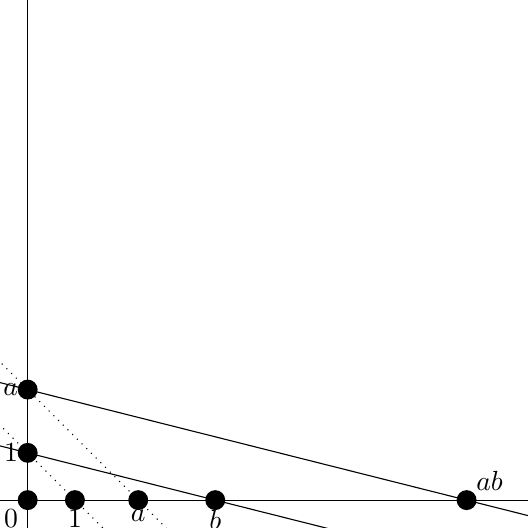
\begin{tikzpicture}[scale=0.6]
  \useasboundingbox (0,0) rectangle (10,10);
  \coordinate (origin) at (0,0);
  \coordinate (x) at (10,0);
  \coordinate (y) at (0,10);

  \draw[->] ($ (origin)!-.1!(x) $) -- ($ (origin)!1.1!(x) $);
  \draw[->] ($ (origin)!-.1!(y) $) -- ($ (origin)!1.1!(y) $);

  \coordinate (one) at (1,0);
  \coordinate (one') at (0,1);

  \pause
  \fill (one) circle (6pt) node[anchor=north] {1};
  \fill (origin) circle (6pt) node[anchor=north east] {0};

  \pause
  \fill (one') circle (6pt) node[anchor=east] {1};

  \pause
  \draw[dotted] ($ (one)!-15!(one') $) -- ($ (one)!15!(one') $);

  \pause
  \coordinate (a) at (2.34,0);
  \coordinate (b) at (3.97,0);
  \coordinate (ab) at (9.2898,0);
  \coordinate (a') at (0,2.34);
  \coordinate (b') at (0,3.97);

  \fill (a) circle (6pt) node[anchor=north] {$a$};
  \fill (b) circle (6pt) node[anchor=north] {$b$};

  \pause
  \draw[dotted] ($ (a)!-15!(a') $) -- ($ (a)!15!(a') $);
%  \draw[dotted] ($ (b)!-15!(b') $) -- ($ (b)!15!(b') $);

  \pause
  \fill (a') circle (6pt) node[anchor=east] {$a$};
%  \fill (b') circle (6pt) node[anchor=east] {$b$};

  \pause
  \draw ($ (b)!-15!(one') $) -- ($ (b)!15!(one') $);

  \pause
  \draw ($ (a')!-15!(ab) $) -- ($ (a')!15!(ab) $);

  \pause
  \fill (ab) circle (6pt) node[anchor=south west] {$ab$};

\end{tikzpicture}
\end{center}

\end{frame}

%%%%%%%%%%%%%%%%%%%%%%%%%%%%%%%%%%%%%%%%%%%%%%%%%%%%%%%%%%%%%%%%
\begin{frame}
\frametitle{How to multiply (in projective plane)}

\begin{center}
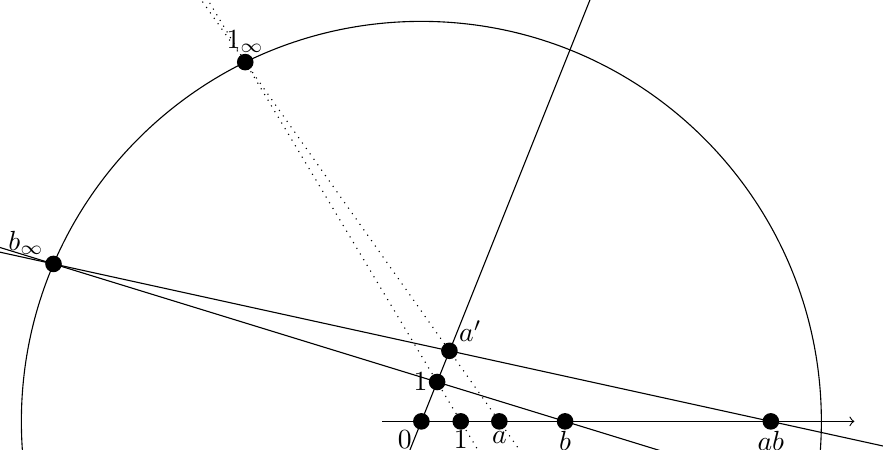
\begin{tikzpicture}[scale=0.5]
  \useasboundingbox (-10,0) rectangle (11,10);
  \coordinate (origin) at (0,0);
  \coordinate (x) at (10,0);
  \coordinate (y) at (4,10);

  \draw[->, name path=x axis] ($ (origin)!-.1!(x) $) -- ($ (origin)!1.1!(x) $);
  \draw[->, name path=y axis] ($ (origin)!-.1!(y) $) -- ($ (origin)!1.1!(y) $);

  \coordinate (one) at (1,0);
  \coordinate (one') at ($ (origin)!0.1!(y) $);

  \draw[name path=circle at infinity] (origin) circle (4in);

  \path [name intersections={of=x axis and circle at infinity, by=x infinity}] ;
  \path [name intersections={of=y axis and circle at infinity, by=y infinity}] ;

  \pause
  \fill (one) circle (6pt) node[anchor=north] {1};
  \fill (origin) circle (6pt) node[anchor=north east] {0};

  \pause
  \fill (one') circle (6pt) node[anchor=east] {1};

  \pause
  \draw[dotted,name path=one line] ($ (one)!-15!(one') $) -- ($ (one)!15!(one') $);

  \path [name intersections={of=one line and circle at infinity, by=one-infinity}] ;
  \fill (one-infinity) circle (6pt) node[anchor=south] {$1_\infty$};

  \pause
  \coordinate (a) at (1.98,0);
  \coordinate (b) at (3.65,0);

  \fill (a) circle (6pt) node[anchor=north] {$a$};
  \fill (b) circle (6pt) node[anchor=north] {$b$};

  \pause
  \draw[dotted,name path=a one line] ($ (a)!-15!(one-infinity) $) -- ($ (a)!15!(one-infinity) $);
  \path [name intersections={of=a one line and y axis, by=a'}] ;
  \fill (a') circle (6pt) node[anchor=south west] {$a'$};

  \pause
  \draw[name path=b line] ($ (one')!-15!(b) $) -- ($ (one')!15!(b) $);
  \path [name intersections={of=b line and circle at infinity, by=b infinity}] ;
  \fill (b infinity) circle (6pt) node[anchor=south east] {$b_\infty$};

  \pause
  \draw[name path=a line] ($ (b infinity)!-15!(a') $) -- ($ (b infinity)!15!(a') $);
  \path [name intersections={of=a line and x axis, by=ab}] ;
  \fill (ab) circle (6pt) node[anchor=north] {$ab$};

\end{tikzpicture}
\end{center}

\end{frame}

\againframe<10>{fano}

%%%%%%%%%%%%%%%%%%%%%%%%%%%%%%%%%%%%%%%%%%%%%%%%%%%%%%%%%%%%%%%%
\begin{frame}
\frametitle{How to divide}
\scriptsize
\begin{center}
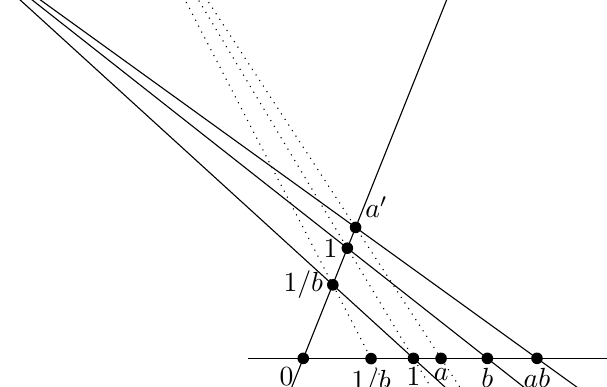
\begin{tikzpicture}[scale=0.7]
  \useasboundingbox (-5,0) rectangle (5,6);
  \coordinate (origin) at (0,0);
  \coordinate (x) at (10,0);
  \coordinate (y) at (4,10);

  \draw[->, name path=x axis] ($ (origin)!-.1!(x) $) -- ($ (origin)!1.1!(x) $);
  \draw[->, name path=y axis] ($ (origin)!-.1!(y) $) -- ($ (origin)!1.1!(y) $);

  \coordinate (one) at (2,0);
  \coordinate (one') at ($ (origin)!0.2!(y) $);

  \draw[name path=circle at infinity] (origin) circle (4in);

  \path [name intersections={of=x axis and circle at infinity, by=x infinity}] ;
  \path [name intersections={of=y axis and circle at infinity, by=y infinity}] ;

  \pause
  \fill (one) circle (3pt) node[anchor=north] {1};
  \fill (origin) circle (3pt) node[anchor=north east] {0};

  \pause
  \fill (one') circle (3pt) node[anchor=east] {1};

  \pause
  \draw[dotted,name path=one line] ($ (one)!-15!(one') $) -- ($ (one)!15!(one') $);

  \path [name intersections={of=one line and circle at infinity, by=one-infinity}] ;
  \fill (one-infinity) circle (3pt) node[anchor=south] {$1_\infty$};

  \pause
  \coordinate (a) at ($ (origin)!0.25!(x) $);
  \coordinate (b) at (3.34,0);

  \fill (a) circle (3pt) node[anchor=north] {$a$};
  \fill (b) circle (3pt) node[anchor=north] {$b$};

  \pause
  \draw[dotted,name path=a one line] ($ (a)!-15!(one-infinity) $) -- ($ (a)!15!(one-infinity) $);
  \path [name intersections={of=a one line and y axis, by=a'}] ;
  \fill (a') circle (3pt) node[anchor=south west] {$a'$};

  \pause
  \draw[name path=b line] ($ (one')!-15!(b) $) -- ($ (one')!15!(b) $);
  \path [name intersections={of=b line and circle at infinity, by=b infinity}] ;
  \fill (b infinity) circle (3pt) node[anchor=south east] {$b_\infty$};

  \pause
  \draw[name path=a line] ($ (b infinity)!-15!(a') $) -- ($ (b infinity)!15!(a') $);
  \path [name intersections={of=a line and x axis, by=ab}] ;
  \fill (ab) circle (3pt) node[anchor=north] {$ab$};

  \pause
  \draw[name path=inverse line] ($ (b infinity)!-15!(one) $) -- ($ (b infinity)!15!(one) $);
  \path [name intersections={of=inverse line and y axis, by=inverse'}] ;
  \fill (inverse') circle (3pt) node[anchor=east] {$1/b$};
  
  \pause
  \draw[dotted,name path=inverse one line] ($ (inverse')!-15!(one-infinity) $) -- ($ (inverse')!15!(one-infinity) $);
  \path [name intersections={of=inverse one line and x axis, by=inverse}] ;
  \fill (inverse) circle (3pt) node[anchor=north] {$1/b$};

\end{tikzpicture}
\end{center}

\end{frame}

%%%%%%%%%%%%%%%%%%%%%%%%%%%%%%%%%%%%%%%%%%%%%%%%%%%%%%%%%%%%%%%%
\begin{frame}[label=distributive-law]
  \frametitle{Distributive law}
  \scriptsize
\begin{center}
\begin{tikzpicture}[scale=0.5]
  \useasboundingbox (-4.5,0) rectangle (8,8);
  \coordinate (origin) at (0,0);
  \coordinate (x) at (15,0);
  \coordinate (y) at (4,15);

  \draw[->, name path=x axis] ($ (origin)!-.1!(x) $) -- ($ (origin)!1.1!(x) $);
  \draw[->, name path=y axis] ($ (origin)!-.1!(y) $) -- ($ (origin)!1.1!(y) $);

  \coordinate (one) at (0.5,0);
  \coordinate (one') at ($ (origin)!0.1!(y) $);

%  \alt<22->{
%    \only<22>{\draw[name path=circle at infinity] (origin) circle (5.0in);}
%    \only<23>{\draw[name path=circle at infinity] (origin) circle (5.5in);}
%    \only<24->{\draw[name path=circle at infinity] (origin) circle (6.0in);}
%  }{
    \draw[name path=circle at infinity] (origin) circle (5in);
%  }

  \path [name intersections={of=x axis and circle at infinity, by=x infinity}] ;
  \path [name intersections={of=y axis and circle at infinity, by=y infinity}] ;

  \pause%2
  \fill (one) circle (3pt) node[anchor=north] {1};
  \fill (origin) circle (3pt) node[anchor=north east] {0};

  \pause%3
  \fill (one') circle (3pt) node[anchor=east] {1};

  \pause%4
  \draw[dotted,name path=one line] ($ (one)!-15!(one') $) -- ($ (one)!15!(one') $);

  \path [name intersections={of=one line and circle at infinity, by=one-infinity}] ;
  \fill (one-infinity) circle (3pt) node[anchor=south] {$1_\infty$};

  \pause%5
  \coordinate (a) at (0.8,0);
  \coordinate (b) at (1.1,0);
  \coordinate (c) at (2.40,0);

  \fill (a) circle (3pt) node[anchor=north] {$a$};
  \fill (b) circle (3pt) node[anchor=north west] {$b$};
  \fill (c) circle (3pt) node[anchor=north] {$c$};

  \pause%6
  \draw[dotted,name path=a one line] ($ (a)!-15!(one-infinity) $) -- ($ (a)!15!(one-infinity) $);
  \path [name intersections={of=a one line and y axis, by=a'}] ;
  \fill (a') circle (3pt) node[anchor=east] {$a'$};

  \pause%7
  \draw[dotted,name path=b one line] ($ (b)!-15!(one-infinity) $) -- ($ (b)!15!(one-infinity) $);
  \path [name intersections={of=b one line and y axis, by=b'}] ;
  \fill (b') circle (3pt) node[anchor=east] {$b'$};

  \pause%8
  \draw[name path=a x infinity] ($ (a')!-15!(x infinity) $) -- ($ (a')!15!(x infinity) $);
  \pause%9
  \draw[name path=b y infinity] ($ (b)!-15!(y infinity) $) -- ($ (b)!15!(y infinity) $);

  \pause%10
  \color{red}
  \path [name intersections={of=a x infinity and b y infinity, by=d}] ;
  \fill (d) circle (3pt) node[anchor=south west] {$d$};

  \pause%11
  \draw[name path=d one line] ($ (d)!-15!(one-infinity) $) -- ($ (d)!15!(one-infinity) $);

  \pause%12
  \path [name intersections={of=d one line and x axis, by=ab}] ;
  \fill (ab) circle (3pt) node[anchor=south] {$a+b$};
  \path [name intersections={of=d one line and y axis, by=ab'}] ;
  \fill (ab') circle (3pt) node[anchor=south] {$a+b$};

  \pause%13
  \color{blue}
  \draw[name path=c line] ($ (one')!-15!(c) $) -- ($ (one')!15!(c) $);
  \path [name intersections={of=c line and circle at infinity, by=c infinity}] ;
  \fill (c infinity) circle (3pt) node[anchor=south east] {$c_\infty$};

  \pause%14
  \color{green}
  \draw[name path=abc line] ($ (c infinity)!-15!(ab') $) -- ($ (c infinity)!15!(ab') $);
  \path [name intersections={of=abc line and x axis, by=abc}] ;
  \fill (abc) circle (3pt) node[anchor=north] {$(a+b)c$};

  \pause%15
  \color{magenta}
  \draw[name path=ac line] ($ (c infinity)!-15!(a') $) -- ($ (c infinity)!15!(a') $);
  \path [name intersections={of=ac line and x axis, by=ac}] ;
  \fill (ac) circle (3pt) node[anchor=north] {$ac$};

  \pause%16
  \color{cyan}
  \draw[name path=bc line] ($ (c infinity)!-15!(b') $) -- ($ (c infinity)!15!(b') $);
  \path [name intersections={of=bc line and x axis, by=bc}] ;
  \fill (bc) circle (3pt) node[anchor=north east] {$bc$};

  \pause%17
  \color{magenta}
  \draw[dotted,name path=ac one line] ($ (ac)!-15!(one-infinity) $) -- ($ (ac)!15!(one-infinity) $);
  \path [name intersections={of=ac one line and y axis, by=ac'}] ;
  \fill (ac') circle (3pt) node[anchor=west] {$ac$};

  \pause%18
  \color{gray}
  \draw[name path=ac x infinity] ($ (ac')!-15!(x infinity) $) -- ($ (ac')!15!(x infinity) $);

  \pause%19
  \draw[name path=bc y infinity] ($ (bc)!-15!(y infinity) $) -- ($ (bc)!15!(y infinity) $);

  \pause%20
  \path [name intersections={of=ac x infinity and bc y infinity, by=e}] ;
  \fill (e) circle (3pt) node[anchor=south west] {$e$};  
  
  \pause%21
  \draw[name path=e one line] ($ (e)!-15!(one-infinity) $) -- ($ (e)!15!(one-infinity) $);

  \pause%22
  \path [name intersections={of=e one line and x axis, by=distributed}] ;
  \fill (distributed) circle (3pt) node[anchor=north] {$ac+bc$};

  \pause%23
  \color{black}
  \draw[dotted,name path=abc one line] ($ (abc)!-15!(one-infinity) $) -- ($ (abc)!15!(one-infinity) $);
  \path [name intersections={of=abc one line and y axis, by=abc'}] ;
  \fill (abc') circle (3pt) node[anchor=west] {$(a+b)c$};

  \pause%24
  \draw[name path=abc' line] ($ (abc)!-15!(ab') $) -- ($ (abc)!15!(ab') $);
  \path [name intersections={of=bc y infinity and abc' line, by=h}] ;
  \fill (h) circle (3pt) node[anchor=south west] {$f$};  

  \pause%25
  \draw[fill opacity=0.5,fill=red] (b') -- (b) -- (bc) -- cycle;
  \draw[fill opacity=0.5,fill=red] (ab') -- (d) -- (h) -- cycle;

  \pause
  \only<26>{
    \draw[line width=6pt,opacity=0.5] ($ (b')!-15!(ab') $) -- ($ (b')!15!(ab') $);
    \draw[line width=6pt,opacity=0.5] ($ (b)!-15!(d) $) -- ($ (b)!15!(d) $);
    \draw[line width=6pt,opacity=0.5] ($ (bc)!-15!(h) $) -- ($ (bc)!15!(h) $);
  }
  
  \pause
  \only<27-28>{
    \draw[red,line width=6pt,opacity=.25] ($ (b')!-15!(b) $) -- ($ (b')!15!(b) $);
    \draw[red,line width=6pt,opacity=.25] ($ (ab')!-15!(d) $) -- ($ (ab')!15!(d) $);
    \draw[green,line width=6pt,opacity=.25] ($ (b)!-15!(bc) $) -- ($ (b)!15!(bc) $);
    \draw[green,line width=6pt,opacity=.25] ($ (d)!-15!(h) $) -- ($ (d)!15!(h) $);
    \draw[blue,line width=6pt,opacity=.25] ($ (ab')!-15!(h) $) -- ($ (ab')!15!(h) $);
    \draw[blue,line width=6pt,opacity=.25] ($ (b')!-15!(bc) $) -- ($ (b')!15!(bc) $);
  }

  \pause%28
  \draw[line width=5pt,opacity=0.5] (x infinity) -- (h) -- (d) -- (a');

  \pause%29
  \draw[fill opacity=0.5,fill=blue] (a') -- (ac) -- (ac') -- cycle;
  \draw[fill opacity=0.5,fill=blue] (h) -- (abc) -- (e) -- cycle;

  \pause%30
  \only<30>{
    \draw[line width=6pt,opacity=0.5] ($ (ac)!-15!(abc) $) -- ($ (ac)!15!(abc) $);
    \draw[line width=6pt,opacity=0.5] ($ (ac')!-15!(e) $) -- ($ (ac')!15!(e) $);
  }

  \pause
  \only<31>{
    \draw[red,line width=6pt,opacity=.25] ($ (a')!-15!(ac) $) -- ($ (a')!15!(ac) $);
    \draw[red,line width=6pt,opacity=.25] ($ (h)!-15!(abc) $) -- ($ (h)!15!(abc) $);
    \draw[green,line width=6pt,opacity=.25] ($ (ac)!-15!(ac') $) -- ($ (ac)!15!(ac') $);
    \draw[green,line width=6pt,opacity=0.5] (abc) -- (e) -- (one-infinity);
    \draw[blue,line width=6pt,opacity=.25] ($ (h)!-15!(e) $) -- ($ (h)!15!(e) $);
    \draw[blue,line width=6pt,opacity=.25] ($ (a')!-15!(ac') $) -- ($ (a')!15!(ac') $);
  }

  \pause%31
  \draw[line width=5pt,opacity=0.5] (abc) -- (e) -- (one-infinity);

% their abc is my cba

  \pause%32
  \node[anchor=center] (conclusion) at (0,-3) {\large and therefore $(a+b)c = ac + bc$};

\end{tikzpicture}
\end{center}

\end{frame}

%%%%%%%%%%%%%%%%%%%%%%%%%%%%%%%%%%%%%%%%%%%%%%%%%%%%%%%%%%%%%%%%
\begin{frame}
  \frametitle{Conclusion}
  \large

  You can recover a division ring \\
  \quad from a projective plane \\
  \quad satisfying Desargues' theorem

  \vfill

  \pause
  
  Division ring?\ldots What about a field?

\end{frame}

%%%%%%%%%%%%%%%%%%%%%%%%%%%%%%%%%%%%%%%%%%%%%%%%%%%%%%%%%%%%%%%%
\begin{frame}<1-11>[label=commutative]
\frametitle{Commutativity of multiplication}
\scriptsize
\begin{center}
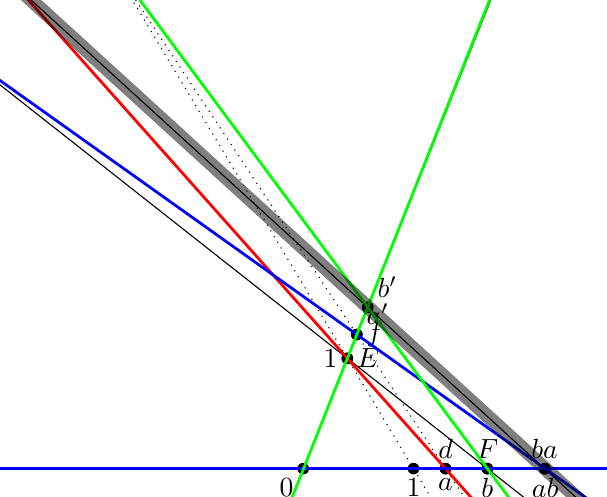
\begin{tikzpicture}[scale=0.7]
  \useasboundingbox (-5,0) rectangle (5,8);
  \coordinate (origin) at (0,0);
  \coordinate (x) at (10,0);
  \coordinate (y) at (4,10);

  \draw[->, name path=x axis] ($ (origin)!-.1!(x) $) -- ($ (origin)!1.1!(x) $);
  \draw[->, name path=y axis] ($ (origin)!-.1!(y) $) -- ($ (origin)!1.1!(y) $);

  \coordinate (one) at (2,0);
  \coordinate (one') at ($ (origin)!0.2!(y) $);

  \draw[name path=circle at infinity] (origin) circle (4in);

  \path [name intersections={of=x axis and circle at infinity, by=x infinity}] ;
  \path [name intersections={of=y axis and circle at infinity, by=y infinity}] ;

  \pause
  \fill (one) circle (3pt) node[anchor=north] {1};
  \fill (origin) circle (3pt) node[anchor=north east] {0};

  \pause
  \fill (one') circle (3pt) node[anchor=east] {1};

  \pause
  \draw[dotted,name path=one line] ($ (one)!-15!(one') $) -- ($ (one)!15!(one') $);

  \path [name intersections={of=one line and circle at infinity, by=one-infinity}] ;
  \fill (one-infinity) circle (3pt) node[anchor=south] {$1_\infty$};

  \pause
  \coordinate (a) at (2.58,0);
  \coordinate (b) at (3.34,0);

  \fill (a) circle (3pt) node[anchor=north] {$a$};
  \fill (b) circle (3pt) node[anchor=north] {$b$};

  \pause
  \draw[dotted,name path=a one line] ($ (a)!-15!(one-infinity) $) -- ($ (a)!15!(one-infinity) $);
  \path [name intersections={of=a one line and y axis, by=a'}] ;
  \fill (a') circle (3pt) node[anchor=south west] {$a'$};

  \pause
  \draw[dotted,name path=b one line] ($ (b)!-15!(one-infinity) $) -- ($ (b)!15!(one-infinity) $);
  \path [name intersections={of=b one line and y axis, by=b'}] ;
  \fill (b') circle (3pt) node[anchor=south west] {$b'$};

  \pause
  \draw[name path=b line] ($ (one')!-15!(b) $) -- ($ (one')!15!(b) $);
  \path [name intersections={of=b line and circle at infinity, by=b infinity}] ;
  \fill (b infinity) circle (3pt) node[anchor=south east] {$b_\infty$};

  \pause
  \draw[name path=a line] ($ (b infinity)!-15!(a') $) -- ($ (b infinity)!15!(a') $);
  \path [name intersections={of=a line and x axis, by=ab}] ;
  \fill (ab) circle (3pt) node[anchor=north] {$ab$};

  \pause
  \draw[name path=a line] ($ (one')!-15!(a) $) -- ($ (one')!15!(a) $);
  \path [name intersections={of=a line and circle at infinity, by=a infinity}] ;
  \fill (a infinity) circle (3pt) node[anchor=south east] {$a_\infty$};

  \pause
  \draw[name path=b line] ($ (a infinity)!-15!(b') $) -- ($ (a infinity)!15!(b') $);
  \path [name intersections={of=b line and x axis, by=ba}] ;
  \fill (ba) circle (3pt) node[anchor=south] {$ba$};

%%%%%%%%%%%%%%%%%%%%%%%%%%%%%%%%%%%%%%%%%%%%%%%%%%%%%%%%%%%%%%%%
      \coordinate (A) at (b infinity);
      \coordinate (B) at (one');
      \coordinate (C) at (b);

      \coordinate (a) at (a);
      \coordinate (b) at (one-infinity);
      \coordinate (c) at (a');

      \pause
      \fill (A) circle (3pt) node[anchor=west] {$D$};
      \fill (B) circle (3pt) node[anchor=west] {$E$};
      \fill (C) circle (3pt) node[anchor=south] {$F$};
      
 %     \pause
 %     \draw[name path=uppercase line] ($ (A)!-15!(C) $) -- ($ (A)!15!(C) $);

%      \pause
      \pause
      \fill (a) circle (3pt) node[anchor=south] {$d$};
      \fill (b) circle (3pt) node[anchor=north] {$e$};
      \fill (c) circle (3pt) node[anchor=west] {$f$};

%      \pause
%      \draw[name path=lowercase line] ($ (a)!-25!(c) $) -- ($ (a)!25!(c) $);
      
      \color{red}
      \pause
%      \draw[line width=1pt,name path=Ab] ($ (A)!-25!(b) $) -- ($ (A)!25!(b) $);
      \draw[line width=1pt,name path=Ab] (origin) circle (4in);
      \draw[line width=1pt,name path=aB] ($ (a)!-25!(B) $) -- ($ (a)!25!(B) $);
      \path [name intersections={of=Ab and aB, by=X}];
%      \fill (X) circle (3pt) node[anchor=north] {$X$};

      \color{blue}
      \pause
      \draw[line width=1pt,name path=Ac] ($ (A)!-25!(c) $) -- ($ (A)!25!(c) $);      
      \draw[line width=1pt,name path=Ca] ($ (C)!-25!(a) $) -- ($ (C)!25!(a) $);      
      \path [name intersections={of=Ac and Ca, by=Y}];
%      \fill (Y) circle (3pt) node[anchor=north] {$Y$};

      \color{green}
      \pause
      \draw[line width=1pt,name path=Bc] ($ (B)!-25!(c) $) -- ($ (B)!25!(c) $);      
      \draw[line width=1pt,name path=bC] ($ (b)!-25!(C) $) -- ($ (b)!25!(C) $);      
      \path [name intersections={of=Bc and bC, by=Z}];
%      \fill (Z) circle (3pt) node[anchor=north] {$Z$};

      \color{black}
      \pause
      \draw[line width=5pt,opacity=0.5] ($ (X)!-25!(Y) $) -- ($ (X)!25!(Y) $);


\end{tikzpicture}
\end{center}

\end{frame}

\begin{frame}[label=pappus]
  \frametitle{Pappus' theorem}

  \begin{center}
    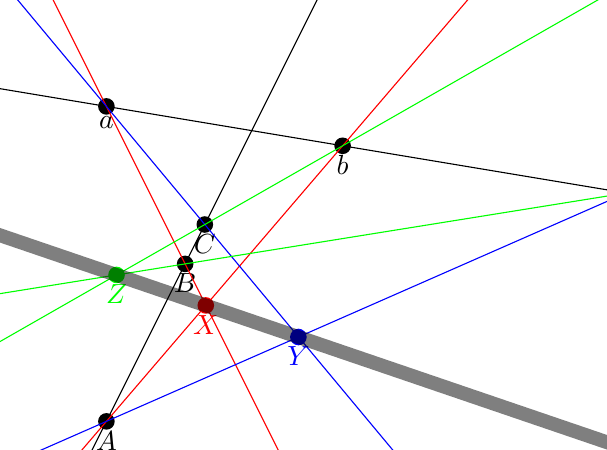
\begin{tikzpicture}
      \useasboundingbox (-2,0) rectangle (5,5);
      \coordinate (A) at (-1,0);
      \coordinate (B) at (0,2);
      \coordinate (C) at ($ (A)!1.25!(B) $);

      \fill (A) circle (3pt) node[anchor=north] {$A$};
      \fill (B) circle (3pt) node[anchor=north] {$B$};
      \fill (C) circle (3pt) node[anchor=north] {$C$};
      
      \pause
      \draw[name path=uppercase line] ($ (A)!-15!(C) $) -- ($ (A)!15!(C) $);

      \pause
      \coordinate (a) at (-1,4);
      \coordinate (b) at (2,3.5);
      \coordinate (c) at ($ (a)!2.2!(b) $);

      \fill (a) circle (3pt) node[anchor=north] {$a$};
      \fill (b) circle (3pt) node[anchor=north] {$b$};
      \fill (c) circle (3pt) node[anchor=north] {$c$};

      \pause
      \draw[name path=lowercase line] ($ (a)!-15!(c) $) -- ($ (a)!15!(c) $);
      
      \color{red}
      \pause
      \draw[name path=Ab] ($ (A)!-15!(b) $) -- ($ (A)!15!(b) $);      
      \draw[name path=aB] ($ (a)!-15!(B) $) -- ($ (a)!15!(B) $);
      \path [name intersections={of=Ab and aB, by=X}];
      \fill (X) circle (3pt) node[anchor=north] {$X$};

      \color{blue}
      \pause
      \draw[name path=Ac] ($ (A)!-15!(c) $) -- ($ (A)!15!(c) $);      
      \draw[name path=Ca] ($ (C)!-15!(a) $) -- ($ (C)!15!(a) $);      
      \path [name intersections={of=Ac and Ca, by=Y}];
      \fill (Y) circle (3pt) node[anchor=north] {$Y$};

      \color{green}
      \pause
      \draw[name path=Bc] ($ (B)!-15!(c) $) -- ($ (B)!15!(c) $);      
      \draw[name path=bC] ($ (b)!-15!(C) $) -- ($ (b)!15!(C) $);      
      \path [name intersections={of=Bc and bC, by=Z}];
      \fill (Z) circle (3pt) node[anchor=north] {$Z$};

      \color{black}
      \pause
      \draw[line width=5pt,opacity=0.5] ($ (X)!-15!(Y) $) -- ($ (X)!15!(Y) $);

    \end{tikzpicture}
  \end{center}

\end{frame}

\againframe{commutative}

\begin{frame}<1-3>[label=hessenberg]
  \frametitle{Pappus implies commutative multiplication}

  So if Pappus' theorem holds, \\
  \quad then the division ring is a field.

  \pause
  \vfill
  \begin{theorem}[Hessenberg]
    Pappus' theorem $\Rightarrow$ Desargues' theorem.
  \end{theorem}
  \begin{proof}
    Three applications of Pappus' theorem.
  \end{proof}

  \vfill\pause

  What about the converse? \pause \textbf{False!}

\end{frame}

\againframe{desargues}

\againframe{pappus}

\againframe<3-4>{hessenberg}

%%%%%%%%%%%%%%%%%%%%%%%%%%%%%%%%%%%%%%%%%%%%%%%%%%%%%%%%%%%%%%%%
% example of division ring
\begin{frame}
  \frametitle{Quaternions}

  A \textbf{quaternion} is 
  $$a + b\quat{i} + c\quat{j} + d\quat{k}$$
  for $a, b, c, d \in \R$.

  \begin{columns}
    \begin{column}{0.3\textwidth}
      \uncover<2->{
        \begin{align*}
          \quat{i} \cdot \quat{i} &= -1 \\
          \quat{j} \cdot \quat{j} &= -1 \\
          \quat{k} \cdot \quat{k} &= -1 \\
        \end{align*}
      }
    \end{column}
    \begin{column}{0.3\textwidth}
      \uncover<3->{
        \begin{align*}
          \quat{i} \cdot \quat{j} &= \quat{k} \\
          \quat{j} \cdot \quat{k} &= \quat{i} \\
          \quat{k} \cdot \quat{i} &= \quat{j} \\
          \quat{j} \cdot \quat{i} &= -\quat{k} \\
          \quat{k} \cdot \quat{j} &= -\quat{i} \\
          \quat{i} \cdot \quat{k} &= -\quat{j} \\
        \end{align*}
      }
    \end{column}
    \begin{column}{0.4\textwidth}
      \uncover<4->{
        \begin{center}
          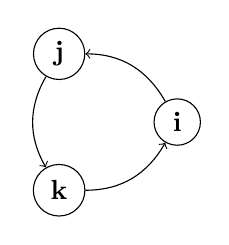
\begin{tikzpicture}
            \node[circle,draw,fill=white] (i) at (0:1cm) {$\quat{i}$};
            \node[circle,draw,fill=white] (j) at (120:1cm) {$\quat{j}$};
            \node[circle,draw,fill=white] (k) at (-120:1cm) {$\quat{k}$};
            \draw [->] (i) edge[out=120,in=0] (j);
            \draw [->] (j) edge[out=240,in=120] (k);
            \draw [->] (k) edge[out=0,in=-120] (i);
          \end{tikzpicture}
        \end{center}
      }
    \end{column}
  \end{columns}

\end{frame}

%%%%%%%%%%%%%%%%%%%%%%%%%%%%%%%%%%%%%%%%%%%%%%%%%%%%%%%%%%%%%%%%
\begin{frame}
  \frametitle{Quaternionic projective plane}

  $\dim_{\mathbb{R}} \mathbb{H}P^2 = 8$.

  \vfill\pause

  $\mathbb{H}P^2$ satisfies Desargues' theorem, \\
  \quad but does not satisfy Pappus' theorem.

  \vfill

\end{frame}


%%%%%%%%%%%%%%%%%%%%%%%%%%%%%%%%%%%%%%%%%%%%%%%%%%%%%%%%%%%%%%%%
% things i should include?
\begin{frame}

  \begin{theorem}[Wedderburn]
    A finite division ring is a field.
  \end{theorem}
  \pause
  \begin{proof}
    Algebra.
  \end{proof}

\end{frame}

\begin{frame}

  \begin{tikzpicture}
    \node (desarguesian) at (0,0) {\parbox{\widthof{projective
          plane}}{\begin{center}\only<2->{finite \\}Desarguesian \\projective
            plane \end{center}}};

    \node (pappus) at (6,0) {\parbox{\widthof{satisfying Pappus' theorem}}{\begin{center}\only<2->{finite \\} Desarguesian \\projective
            plane \\ satisfying Pappus' theorem\end{center}}};

    \node (divisionring) at (0,-5) {\parbox{\widthof{division ring}}{%
          \begin{center}\only<2->{finite \\}division
            ring \end{center}}};

    \node (field) at (6,-5) {\parbox{\widthof{finite}}{%
          \begin{center}\only<2->{finite \\}field \end{center}}};

    \draw [<->] (desarguesian) -- (divisionring);

    \draw [<->] (pappus) -- (field);

    \only<3->{
      \draw [<->] (divisionring) -- node[anchor=south] {(Wedderburn)} (field);
    }

  \end{tikzpicture}

\end{frame}

\begin{frame}
  \begin{theorem}
    A finite projective plane \\
    \quad satisfying Desargues' theorem \\
    \quad also satisfies Pappus' theorem.
  \end{theorem}
  \pause
  \begin{proof}
    Finite division rings are finite fields,\\
    \quad by Wedderburn.
  \end{proof}
  \pause
  \vfill
  \textbf{A geometric result without\\
    \quad a ``geometric'' proof.}

\end{frame}

\begin{frame}
  \frametitle{Next steps}

  \vfill

  \begin{center}
    Non-Desarguesian projective planes?
  \end{center}
  
  \vfill
\end{frame}

\begin{frame}
  \frametitle{Corollary}

  A finite Desarguesian projective plane \\
  \quad has $N^2 + N + 1$ points,\\
  \quad for $N = $ prime power.

  \vfill\pause

  \begin{theorem}[Gaston Tarry]
    There is no (non-Desarguesian) projective plane \\
    \quad with $6^2 + 6 + 1 = 43$ points.
  \end{theorem}

  \vfill\pause

  \begin{theorem}[Lam with computer]
    There is no (non-Desarguesian) projective plane \\
    \quad with $10^2 + 10 + 1 = 111$ points.
  \end{theorem}

\end{frame}

%%%%%%%%%%%%%%%%%%%%%%%%%%%%%%%%%%%%%%%%%%%%%%%%%%%%%%%%%%%%%%%%
 \clearbackgroundpicture
\begin{frame}[label=why-me]
  \vfill
  \begin{center}
  \scalebox{2}{\Huge Why me?}
  \end{center}
  \vfill
\end{frame}

\begin{frame}[label=no-three-in-line]
  \frametitle{Undergraduate research project}
  
  \vfill
  
  \textbf{The no-three-in-line problem in a group} \\
  (F--Andrew Groot--Deven Pandya--Bart Snapp)

  \vfill\pause

  Find maximum size of a no-three-in-coset subset of
  $$\mathbb{Z}_p \times \mathbb{Z}_{p^2}$$
  among other abelian groups.

  \vfill
  
\end{frame}

\begin{frame}[nofills,label=rational-projective-planes]

  \begin{theorem}[Adams]
    If a simply-connected manifold $X$ satisfies $H^\star(X; \Z) =
    \Z[x]/(x^3)$, then $\dim X = 4, 8, 16$.    
  \end{theorem}

  \pause%2
  \vfill

  A \textbf{rational projective plane} is  \\
  \quad a smooth manifold $M^{4k}$ \\
  \quad with $H^\star(X;\Q) = \Q[x]/(x^3)$ and $|x| = 2k$. \\

  \pause%3
  \vfill

  \begin{theorem}[F--Zhixu Su]
    If $M^n$ is a rational projective plane, \\
    \quad then $n = 2^a + 2^b$ for integers $a$ and $b$.
  \end{theorem}  
  
  \pause%4
  \vfill

  There is a 32-dimensional rational projective plane.
  
  \pause %5
  \uncover<5-7>{No 
    \alt<5>{$64$}{\alt<6>{$2^{14}$}{$2^{24}$}}-dimensional rational projective plane.}
  
\end{frame}


%%%%%%%%%%%%%%%%%%%%%%%%%%%%%%%%%%%%%%%%%%%%%%%%%%%%%%%%%%%%%%%%
 \clearbackgroundpicture
 \begin{frame}[nofills,label=thanks]
   \vfill
   \begin{center}
   \Huge
    \scalebox{1.5}{\textbf{Thank You}}
   \end{center}
   \vfill

   \LaTeX\ source at \\
     \scalebox{0.85}{\texttt{https://github.com/kisonecat/projective-planes/}}

   \vfill
   
\includegraphics[width=1in]{cc-logo.pdf}
   \hfill\footnotesize\scalebox{0.8}{licensed for reuse under a Creative Commons BY-NC-SA License}
   \null
 \end{frame}


\end{document}
